\documentclass[]{article}

%opening
\title{The effects of attitudes towards risk and ambiguity on educational investment: Preliminary results}
\author{Chau Pham}
%\date{} for no date shown
\usepackage{amsmath, amsfonts, amssymb, amsthm, mathtools, mathrsfs}
\usepackage[margin = 1.0in]{geometry}
\usepackage{bbold, soul}
\usepackage{tgpagella}
\usepackage{braket, setspace, parskip, enumitem}
\usepackage[colorlinks, citecolor = blue]{hyperref}
\usepackage[nameinlink, noabbrev]{cleveref}
\usepackage{caption}
%\usepackage{threeparttable, makecell, cellspace, multirow, booktabs}
\usepackage{verbatim}
\usepackage{natbib}

%---- Simple table template
\begin{comment} 
	\begin{table}[!htbp]\centering
		\begin{threeparttable}
			\setlength{\extrarowheight}{0.2em}
			\begin{tabular}
				content...
			\end{tabular}
			%\caption{text}
			%\label{key}
		\end{threeparttable}
	\end{table}
\end{comment}

%\setlist[enumerate]{label=(\roman*)}

%\setlength{\parindent}{0pt}

\captionsetup[figure]{labelfont=bf}

\begin{document}

\maketitle
\onehalfspacing

\section{Data \& methodology}
I use data from the Longitudinal Internet Studies for the Social Sciences (LISS panel), which is representative of the Dutch population, and the American Life Panel (ALP), which is representative of the American population. Both datasets contain administrative data as well as survey questions designed for the elicitation of risk and ambiguity attitudes.\footnote{For LISS panel, survey number 44 contains said questions on risk and ambiguity. The ALP counterpart is survey number 243.}

\subsection{Survey questions on risk and ambiguity}
To elicit ambiguity aversion, \citet{DIMMOCK2016559, dimmock2016ambiguity} designed special surveys as part of ALP and LISS panel respectively. Specifically, each individual are asked whether they prefer the risky box, the ambiguous box or either (meaning indifferent) as in \Cref{fig:1}.

\begin{figure}[!ht]
	\setlength{\fboxrule}{1.5pt}
	\setlength{\fboxsep}{0pt}
	\fbox{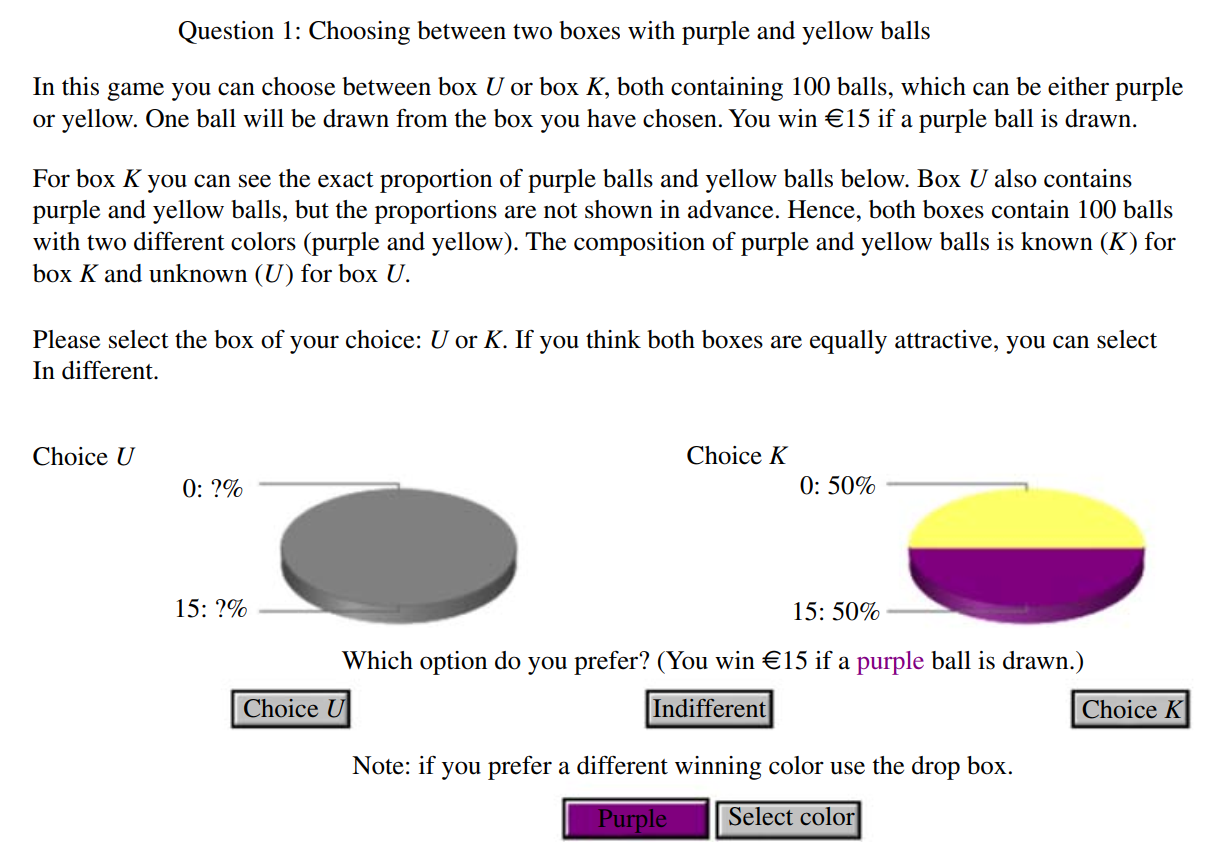
\includegraphics[width=\linewidth]{Figure/figure-1.png}}
	\caption{Question 1 in the ambiguity sequence of the LISS panel.}
	\label{fig:1}
\end{figure}

The question will be asked repeatedly until the respondent chooses "Indifferent" or until the 6th iteration whichever occurs first. \Cref{fig:1} shows the first question in the sequence. If the respondent chooses "Choice U" in this question, she is then presented with a similar question wherein Choice U stays the same while the number of the winning balls in Choice K increases using a bisection method.\footnote{After each question that the respondent chooses either "Choice K" or "Choice U", the proportion of the winning balls in the risky choice is adjusted as follows. In the first question, if "Choice K" is chosen, the proportion of winning ball in the next question is then $(0\% + 50\%)/2 = 25\%$ and $50\%$ becomes the new ceiling instead of $100\%$. If "Choice U" is chosen, the proportion of winning ball in the next question is $(50\% + 100\%)/2 = 75\%$ and $50\%$ becomes the new floor. The new floor and ceiling are carried to the next question and get updated again depending on the subsequent choices of the respondent.} If, on the other hand, "Choice K" is chosen in the first question, in the following question, the number of winning balls in Choice K is reduced. If "Indifferent" is chosen at any stage of the sequence, the sequence stops and the proportion of winning balls in the last stage indicates probability of winning a risky `lottery' that makes the risky choice and ambiguous choice equally attractive. Finally, if "Indifferent" is never chosen, the sequence stops after the 6th iteration of the question and the final probability of winning a risky `lottery' is adjusted via the bisection method. 

In a similar manner, to elicit risk attitudes, a sequence of questions about two choices involving sure gain on one side and a risky lottery on the other are presented to respondents. \Cref{fig:2} shows the first question in this sequence of questions on risk for the ALP. Depending on the choices of the respondent, the amount of sure gain Box A is updated via a bisection method while the risky Box B remains the same. The question is repeated until "Indifferent" is chosen or until the 4th iteration is reached.

\begin{figure}[!ht]
	\setlength{\fboxrule}{1.5pt}
	\setlength{\fboxsep}{0pt}
	\fbox{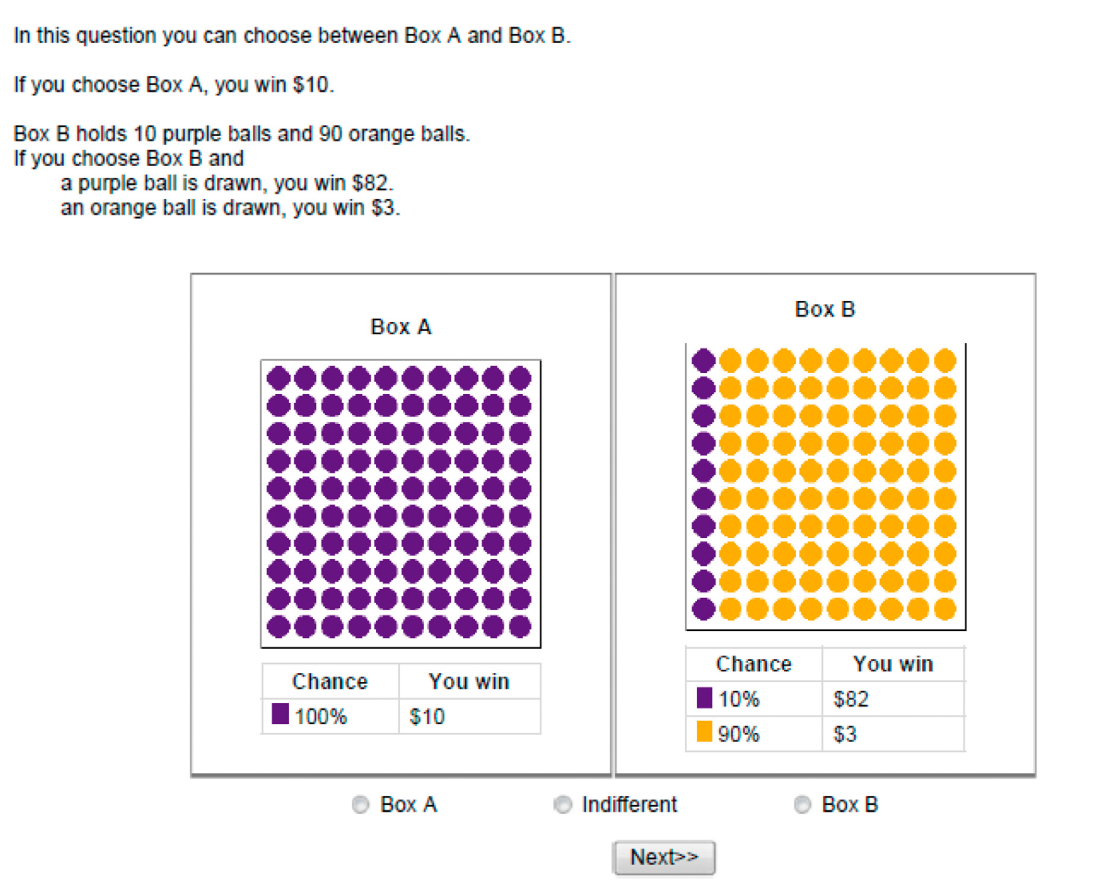
\includegraphics[width = \linewidth]{Figure/figure-2.png}}
	\caption{A randomized question in the risk sequence of ALP.}
	\label{fig:2}
\end{figure} 



\subsection{Elicitation of attitudes towards risk and ambiguity}










\pagebreak
\bibliographystyle{apalike}
\bibliography{bibliography.bib}

\end{document}
